\subsection{Summary of the Exoplanet Catalog}

The final DR25 KOI catalog, available at NExScI contains all of the planet candidates and all TCEs that did not fail due to one of the not-transit like tests (\S\ref{s:ntl}). A summary of the planet radii and period of the planet candidates available in this catalog can be seen in Figure~\ref{f:catalogPlot}. The deficit of planets near 1.8\,R$_{p}$ is consistent with the study of \citet{Fulton2017} where they see a natural gap in the abundance of planets between super-Earths and sub-Neptunes by obtaining precise stellar parameters. A clear excess of candidates exists for PCs with periods near to 370\,d.  After a score cut, this excess disappears. While we have provided an easy way to make additional cuts on the PC population of the catalog with the disposition score, when discussing the PC population here we are using the pure dispositions of the Robovetter unless otherwise stated.


\begin{figure*}
    \centering
    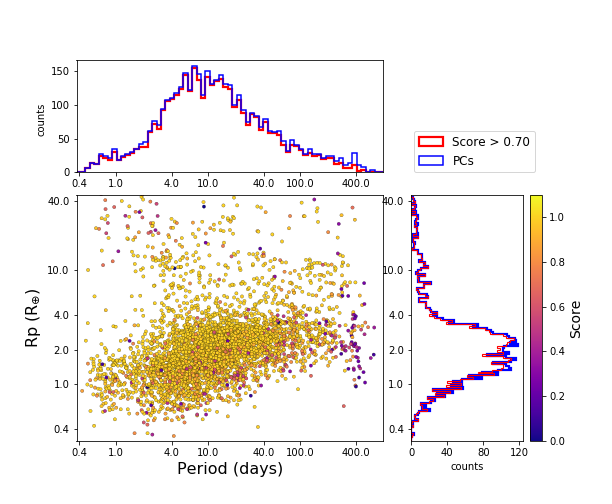
\includegraphics[width=0.9\linewidth]{fig-radiusPeriodScore-hist.png}
    \caption{DR25 Exoplanet Candidates plotted as planet radius against Period with the color representing the disposition score. Those plotted in orange and yellow are those whose metrics lie near to the lest confident PCs.  The period and planet radii distributions are plotted on the top and on the left, respectively, in blue. The red line shows the distributions if you only consider those KOIs with a score greater than 0.8. }
    \label{f:catalogPlot}
\end{figure*}

To summarize, some key stats of the DR25 KOI catalog are as follows:
\begin{itemize}
    \item 8054 KOIs
    \item 4034 Planet Candidates
    \item 1762 KOIs identified as likely eclipsing binaries.
    \item 85 per cent overall completeness
    \item 97 per cent overall reliability
\end{itemize}




\begin{itemize}
    \item [o] plot of pradius vs. period and/or pradius vs insol. flux
    \item [o] Histogram of number of candidates of different sizes (short and long period)
    \item [o] Discuss number of candidates compared to previous catalogs.
    \item [o] Discuss identified EBs.
    \item [o] From looking at distributions obvious over abundance at 370 days.
\end{itemize}